\chapter{Multivariable Calculus}

\textbf{Colley (2012)} refers to \textit{Vector Calculus, Fourth Edition} by Susan Jane Colley.

\section{Vectors, lines, planes}

\subsection{$\Real^n$}

\begin{definition}[Two-dimensional real-coordinate space ($\Real^2$)] 
  \[
    \Real^2 = \{ (x, y) : x, y \in \Real \}
  \]
\end{definition}

\begin{definition}[Three-dimensional real-coordinate space ($\Real^2$)] 
  \[
    \Real^3 = \{ (x, y, z) : x, y, z \in \Real \}
  \]

  $x, y, z$ should be presented such that the coordinate system is right-handed ($\khat = \ihat \crossp \jhat$ should have direction according to the right-hand rule).
\end{definition}

\begin{definition}[Standard basis vectors] The standard basis vectors of a space are the unit vectors that go along the axes of the space. All vectors in that space can be expressed as sums of scalar multiples of the standard basis vectors of that space.

The standard basis vectors of $\Real^2$ are $\ihat$ and $\jhat$, also called $\mathbf{e_1}$ and $\mathbf{e_2}$.

The standard basis vectors of $\Real^3$ are $\ihat$, $\jhat$, and $\khat$, also called $\mathbf{e_1}$, $\mathbf{e_2}$, and $\mathbf{e_3}$.
\end{definition}

\subsection{Vectors}

See the properties of fields in the LinAlg notes for definitions of addition and scalar multiplication.

\begin{definition}[Displacement vector]
  The vector from the end of $\vec{A}$ to the end of $\vec{B}$ when their starts are in the same location.

  \[
    \longvec{AB} = \vec{B} - \vec{A}
  \]
\end{definition}

\subsection{Dot and cross products}

\begin{definition}[Dot product]
  Where $a, b \in \Real^n$ and $\theta$ is the angle between $a$ and $b$:
  \[
    a \dotp b = \sum a_i b_i = |a| |b| \cos \theta
  \]
\end{definition}

\begin{theorem}[Properties of dot product]
  For $\vec{a}, \vec{b}, \vec{c} \in \Real^n$ and $k \in \Real$:
  \begin{itemize}
    \item $\vec{a} \dotp \vec{a} = |\vec{a}|^2$
    \item $\vec{a} \dotp \vec{a} = 0$ iff $\vec{a} = 0$
    \item Commutativity: $\vec{a} \dotp \vec{b} = \vec{b} \dotp \vec{a}$
    \item Distributivity: $\vec{a} \dotp (\vec{b} + \vec{c}) = \vec{a} \dotp \vec{b} + \vec{a} \dotp \vec{c}$
    \item Distributivity: $(k \vec{a}) \dotp b = k(\vec{a} \dotp \vec{b}) = a \dotp (k \vec{b})$
    \item $\vec{a} \dotp \vec{b} = 0$ iff $a \perp b$, $a = 0$, or $b = 0$.
  \end{itemize}
\end{theorem}

\begin{definition}[Cross product]
  For $\vec{a}, \vec{b} \in \Real^3$, the unique vector $a \crossp b$ satisfying
  \begin{itemize}
    \item $|a \crossp b|$ is the area of the parallelogram spanned by $a$ and $b$
    \item $a \crossp b = 0$ iff $a \parallel b$, $a = 0$, or $b = 0$.
    \item $a \crossp b$ is orthogonal to $a$ and $b$.
    \item $(a, b, a \crossp b)$ is right-handed (if the coordinate system is right-handed)
  \end{itemize}
\end{definition}

\begin{theorem}[Properties of cross product]
  For $a, b, c \in \Real^3$ and $k \in \Real$:
  \begin{itemize}
    \item $a \crossp b = (-b) \crossp a$
    \item $a \crossp (b + c) = a \crossp b + a \crossp c$
    \item $(a + b) \crossp c = a \crossp c + b \crossp c$
    \item $k(a \crossp b) = (ka) \crossp b = a \crossp (kb)$
  \end{itemize}
\end{theorem}

\begin{theorem}[Calculation of cross product]
  Where $a, b \in \Real^n$ and $\theta$ is the angle between $a$ and $b$:
  \begin{align*}
    a \crossp b &= \begin{bmatrix}
      a_2 b_3 - a_3 b_2 \\
      a_3 b_1 - a_1 b_3 \\
      a_1 b_2 - a_2 b_1 \\
    \end{bmatrix} = \begin{vmatrix}
      \ihat & \jhat & \khat \\
      a_1 & a_2 & a_3 \\
      b_1 & b_2 & b_3
    \end{vmatrix} \\
    &= \ihat \begin{vmatrix}
      a_2 & a_3 \\
      b_2 & b_3
    \end{vmatrix}
    + \jhat \begin{vmatrix}
      a_1 & a_3 \\
      b_1 & b_3
    \end{vmatrix}
    + \khat \begin{vmatrix}
      a_1 & a_2 \\
      b_1 & b_2
    \end{vmatrix}
  \end{align*}
  \[
    |a \crossp b| = |a| |b| \sin \theta
  \]
\end{theorem}

\subsection{Lines}

The most useful notation for a line is in parametric form:

\begin{definition}[Parametric form of a line]
  Where $r_0 \in \Real^3$ is a point on the line, and $t \in \Real^3$:
  \[
    r(t) = r_0 + vt
  \]

  $t$ is called the \textbf{direction vector}.
\end{definition}

\begin{theorem}
  Two lines are parallel iff their direction vectors are scalar multiples of each other.
\end{theorem}

\begin{definition}[Skew lines]
  Two lines are skew iff they do not intersect but are not parallel, i.e. they lie in different parallel planes.
\end{definition}

\begin{procedure}[Finding the intersection of two lines]
  Given lines with parametric equations
  \[
    r_1(t) = a_1 + v_1 t \qquad r_2(t) = a_2 + v_2 t
  \]
  solve the system of equations
  \[
    a_1 + v_1 t_1 = a_2 + v_2 t_2
  \]
  for $t_1$ or $t_2$, then plug it in to the appropriate equation.

  (Break up the equation into its $x$, $y$, and $z$ components, or whichever is appropriate for your coordinate space.)
\end{procedure}

\subsection{Planes}

\refresources{Colley [1.5]}

\begin{definition}[Plane]
  A plane $\Pi$ is determined uniquely by a point $P$ in the plane and a normal vector $n$.

  A plane is the set of points $A$ in space such that $\vec{AP}$ is perpendicular to $n$.
\end{definition}

\begin{theorem}[Scalar equation for a plane in $\Real^3$]
  If $n \in \Real^3$ is the \textbf{normal vector} to the plane (vector perpendicular to the plane), and $P \in \Real^3$ is a point on the plane:

  \[
    n_x (x - P_x) + n_y (x - P_y) + n_z (z - P_z) = 0
  \]

  or equivalently:

  \[
    n_x x + n_y y + n_z z = n_x P_x + n_y P_y + n_z P_z
  \]
\end{theorem}

\begin{procedure}[Equation of plane containing three points]
  If $A, B, C \in \Real^3$ are points on our plane, then we can find the normal vector by performing $n = \longvec{AB} \crossp \longvec{AC} = (B - A) \crossp (C - A)$ (since $\longvec{AB}$ and $\longvec{AC}$ are vectors on the plane).
\end{procedure}

\begin{theorem}[Parametric equation for a plane in $\Real^3$]
  If $a, b \in \Real^3$ are nonparallel nonzero vectors on the plane, and $P \in \Real^3$ is a point on the plane, then the parametric equation for the plane is:
  \[
    x(s, t) = P + sa + tb
  \]
\end{theorem}

\subsection{Distance}

\refresources{Colley [1.5]}

\begin{procedure}[Distance between point and line]
  Let $P$ be the point, and $A + Lt$ be the line. Then the distance is
  \[
    |\longvec{AP} - \proj_L \longvec{AP}| = \vec{P}
  \]
\end{procedure}

\begin{procedure}[Distance between parallel planes]
  Let $\Pi_1$ and $\Pi_2$ be the two planes.

  If $n$ is normal to both planes, and $P_1 \in \Pi_1$ and $P_2 \in \Pi_2$, then the answer is
  \[
    |\proj_n \longvec{P_1 P_2}
  \]
\end{procedure}

\subsection{Cylindrical and spherical coordinates}

\refresources{Colley [1.7] Trimm [5.6, 5.7] \\
Brummet [08, MVCWUP:Feb3(29-33)]}

\begin{definition}[Cylindrical coordinate]
  An ordered pair $(r, \theta, z)$ where $r$ is the distance between the point and the $z$-axis, $\theta$ is the angle counterclockwise from the positive $x$-axis along the $xy$-plane, and $z$ is the position on the $z$-axis.
\end{definition}

\begin{definition}[Spherical coordinate]
  An ordered pair $(\rho, \phi, \theta)$, where $\rho$ is the distance between the point and the origin, $\phi$ is the angle clockwise from the positive $z$-axis going downwards towards the $xy$-plane, and $\theta$ is the angle counterclockwise from the positive $x$-axis along the $xy$-plane.

  Typically we use the following restrictions:
  \[
    \rho > 0 \qquad 0 \leq \theta \leq 2\pi \qquad 0 \leq \phi \leq \pi
  \]
\end{definition}

\begin{theorem}[Useful formulas]
  \[
    r = \rho \sin \phi \qquad z = \rho \cos \phi \qquad
  \]\[
    x = \rho \sin \phi \cos \theta \qquad y = \rho \sin \phi \sin \theta
  \]\[
    r^2 = x^2 + y^2 \qquad x = r \cos \theta \qquad y = r \sin \theta
  \]
\end{theorem}

\section{Functions, limits, differentiation}

\subsection{Multivariable functions}

\refresources{Colley [2.1] Trimm [3.1, 3.2] Brummet [MVCWUP:Feb4(35-41)]}

\begin{definition}[Function]
  All functions $f : X \to Y$ are defined by:
  \begin{itemize}
    \item A domain set $X$
    \item A codomain set $Y$
    \item A rule of assignment that associates a unique element $y \in Y$ to each element $x \in X$
  \end{itemize}
\end{definition}

\begin{definition}[Graph]
  The graph of $f : X \subseteq \Real^n \to \Real$ is the set
  \[
    \{(x_1, \ldots, x_n, f(x)) : x = (x_1, \ldots, x_n)\}
  \]
  Specifically, for $f : \Real^2 \to \Real$ the graph is the set
  \[
    \{(x, y, z) : (x, y) \in X \text{ and } z = f(x, y)\}
  \]
\end{definition}

\begin{definition}[Level set]
  Let $f : X \subseteq \Real^n \to \Real$. The \textbf{level set at height $c$ of $f$} is the set in $\Real^n$ defined by the equation $f(\vec{a}) = c$, where $c$ is a constant. This is equivalent to the set
  \[
    \{ \vec{x} \in \Real^n : f(\vec{x}) = c \}
  \]

  In $\Real^2$, this is also called a \textbf{level curve}.
\end{definition}

\begin{definition}[Contour set]
  Let $f : X \subseteq \Real^n \to \Real$. The \textbf{contour set at height $c$ of $f$} is the set in $\Real^{n + 1}$ defined by the two equations $z = f(\vec{a})$ and $z = c$, where $c$ is a constant. This is equivalent to the set
  \[
    \{ \vec{x} \in \Real^{n + 1} : z = f(\vec{x}) = c \}
  \]

  If $f : X \subseteq \Real^2 \to \Real$, this is also called a \textbf{contour curve}. It is equivalent to the level curve, except it is located in $\Real^3$ rather than $\Real^2$.
\end{definition}

% TODO: finish this

\subsection{Limits}

\refresources{Trimm [3.3, DiffEq-1.0] Brummet [09, MVCWUP:Feb11(42-46)] \\
Colley [2.2]}

\begin{definition}[Limit]
  $\lim_{\vec{x} \to \vec{a}} f(\vec{x}) = \vec{L}$ if for all $\varepsilon > 0$, there exists $\delta > 0$ s.t. if $0 < |\vec{x} - \vec{a}| < \delta$ then $|f(\vec{a}) - \vec{L}| < \varepsilon$.
\end{definition}

\begin{definition}[Continuity]
  Let $f : X \subseteq \Real^n \to \Real^m$ and let $\vec{a} \in X$. Then $f$ is continuous at point $\vec{a}$ iff
  \[
    \lim_{\vec{x} \to \vec{a}} f(\vec{x}) = f(\vec{a})
  \]
  If $f$ is continuous at all $\vec{a} \in X$, then we say that $f$ is continuous.
\end{definition}

\subsection{Differentiation}

\refresources{Colley [2.3, 2.4] \\
Trimm [3.4, DiffEq-1.0] \\
Brummet [11, 12.5, MVCWUP:Feb12/22(48-54)]}

\begin{definition}[Partial derivative with respect to $x$]
  The partial derivative of $f(x, y)$ with respect to $x$ is
  \[
    \lim_{h \to 0} \frac{f(a + h, b) - f(a, b)}{h}
  \]

  Let $z = f(x, y)$. Then the partial derivative is denoted by
  \[
    f_x(x, y) = f_x = \frac{\partial f}{\partial x} = \frac{\partial}{\partial x} f(x, y) = \frac{\partial z}{\partial x} = D_x f
  \]
\end{definition}

\begin{definition}[Partial derivative]
  The partial derivative of $f(\vec{x})$ with respect to the $i$th variable is
  \[
    \frac{\partial f(\vec{x})}{\partial x_i} = \lim_{h \to 0} \frac{f\left(\begin{bmatrix}
      x_0 \\
      \vdots \\
      x_i + h \\
      \vdots \\
      x_n
    \end{bmatrix}\right) - f\left(\vec{x}\right)}{h}
  \]

  This is equivalent to letting $F(x_i) = f(\vec{x})$ and finding $F'(x_i)$.
\end{definition}

\begin{definition}[Higher-order partial]
  The result of taking the partial derivative of a partial derivative, which may be higher-order.

  A partial derivative that is not higher-order is called a \textbf{first-order partial}. A partial derivative of a first-order partial is a second-order partial, a partial derivative of a second-order partial is a third-order partial, etc.

  A higher-order partial which is the result of taking the partial with respect to $x_1$, then with respect to $x_2$, then with respect to $x_3, \ldots, x_n$, is denoted by
  \[
    f_{x_1 \cdots x_n} = \frac{\partial}{\partial x_n} \cdots \frac{\partial}{\partial x_1} f
  \]

  $x_1 \cdots x_n$ do not have to be distinct. If $x_1 \cdots x_n$ are not all the same then the higher-order partial is called a \textbf{mixed partial derivative}.
\end{definition}

\begin{definition}[$C^k$ function]
  Where $k$ is a nonnegative integer, a function $f : X \in \Real^n \to \Real$ is of order $C^k$ at point $\vec{x} \in X$ iff its $k$-th order and lower partials exist and are continuous at $\vec{x}$. 

  It is of order $C^\infty$ at point $\vec{x}$ iff it is of order $C^k$ at $\vec{x}$ for all $k \in \Natural$.
  
  It is of order $C^k$ iff it is of order $C^k$ at all $x \in \vec{x}$.
\end{definition}

\begin{theorem}
  Let $f : X \in \Real^n \to \Real$ whose $k$-th order and lower partials exist and are continuous on $X$. Then its $k$-th order and lower partials may be evaluated in any order, i.e.
  \[
    f_{x_1 \cdots x_n} = f_{x_n \cdots x_1} = f_{x_1 x_3 x_{27} \cdots x_4} = \cdots
  \]
\end{theorem}

\begin{definition}[Gradient]
  \[
    \grad f(\vec{x}) = \begin{bmatrix}
      \frac{\partial f(x)}{\partial x_1} \\
      \vdots \\
      \frac{\partial f(x)}{\partial x_n}
    \end{bmatrix}
  \]
\end{definition}

\subsection{Implicit surfaces}

\refresources{Brummet [12]}

\begin{definition}[Implicit surface]
  A surface in $\Real^3$ defined by an equation which is not solved for $x$, $y$, nor $z$.

  We often express it as
  \[
    F(x, y, z) = 0,
  \]
  in which case the surface is the set of points which satisfy $F(x, y, z) = 0$.
\end{definition}

\begin{theorem}
  The gradient $\grad F(\vec{x})$ is the normal vector to the tangent plane to the implicit surface defined by $F(\vec{x}) = k$, where $k$ is a constant.

  Equivalently, if $x_0$ is a point on the level set $S = \{ x \in X : F(x) = k \}$ where $F : X \subseteq \Real^n \to \Real$, then the vector $\grad F(x_0)$ is perpendicular to $S$.
\end{theorem}

\subsection{Chain rule}

\refresources{Colley [2.5] Trimm [3.8, 6.5, DiffEq-1.0] \\
Brummet [12, MVCWUP:Feb24(58-61)]}

\begin{definition}[Jacobian]
  If $f: X \subseteq \Real^n \to \Real^m$ is a vector-valued function, then the Jacobian is
  \[
    Df\left(\begin{bmatrix}
      x_1 \\
      x_2 \\
      \vdots \\
      x_n
    \end{bmatrix}\right) = \begin{bmatrix}
      \grad f_1 \\
      \grad f_2 \\
      \vdots \\
      \grad f_m
    \end{bmatrix} = \begin{bmatrix}
      \frac{\partial f_1}{\partial x_1} & \frac{\partial f_1}{\partial x_2} & \hdots & \frac{\partial f_1}{x_n} \\
      \frac{\partial f_2}{\partial x_1} & \frac{\partial f_2}{\partial x_2} & \hdots & \frac{\partial f_2}{x_n} \\
      \vdots & \vdots & \ddots & \vdots \\
      \frac{\partial f_m}{\partial x_1} & \frac{\partial f_m}{\partial x_2} & \hdots & \frac{\partial f_m}{x_n} \\
    \end{bmatrix}
  \]
\end{definition}

\begin{theorem}[Multivariable chain rule]
  Suppose $X \subseteq \Real^m$ and $T \subseteq \Real^n$ are open and $f : X \to \Real^p$ and
  $r : T \to \Real^m$ are defined so that $T \subseteq X$. If $x$ is
  differentiable at $t_0 \in T$ and f is differentiable at $x_0 = r(t_0)$, then
  the composite $f \compose r$ is differentiable at $t_0$, and we have
  \[
    (f \compose r)'(t) = \grad f(x_0) \dotp r'(t_0)
  \]
  Equivalently,
  \[
    D(f \compose r)(t_0) = Df(x_0) Dr(t_0)
  \]

  In $\Real^3$,
  \[
    \frac{dF}{dt} = \frac{\partial F}{\partial x} \frac{dx}{dt} + \frac{\partial F}{\partial y} \frac{dy}{dt} + \frac{\partial F}{\partial z} \frac{dz}{dt}
  \]
\end{theorem}

\subsection{Paths}

\refresources{Brummet [MVCWUP:Feb24(55-56)]}

\begin{definition}[Path]
  A path in $\Real^n$ is a function $x : I \to \Real^n$, where $I$ is a set of scalars. If $I = [a, b]$, then the endpoints of the path are $f(a)$ and $f(b)$.
\end{definition}

\begin{definition}[Tangent vector]
  Given a path $r : \Real \to \Real^3$, the tangent vector to said path at some point $P$ is given by $r'(t)$, provided that $r'(t) \neq 0$. In $\Real^3$,
  \[
    r'(t) = \lim_{h \to 0} \frac{r(t + h) - r(t)}{h} = \begin{bmatrix}
      \frac{dx}{dt} \\
      \frac{dy}{dt} \\
      \frac{dz}{dt}
    \end{bmatrix}
  \]
\end{definition}

\begin{definition}[Derivative of vector-valued function]
  Let $f : T \subseteq \Real \to \Real^m$. Then
  \[
    f'(t) = \begin{bmatrix}
      f_1'(t) \\
      f_2'(t) \\
      \vdots \\
      f_m'(t) \\
    \end{bmatrix}
  \]
\end{definition}

\subsection{Differentiability}

\refresources{Colley [2.3]
Trimm [3.5] 
Brummet [13.5]}

\begin{definition}[Linear approximation ($\Real^n \to \Real$)]
  The \textbf{linear approximation} or \textbf{tangent plane ($\Real^3$) or hyperplane} to the graph of a function $f$ at the point $\vec{a}$ is expressed by
  \[
    L(\vec{x}) = f(\vec{a}) + \grad f(\vec{a}) \dotp (\vec{x} - \vec{a})
  \]

  In $\Real^3$, this is equivalent to the plane
  \[
    z = L(x, y) = f(a, b) + f_x(a, b) (x - a) + f_y(a, b) (y - b)
  \]
\end{definition}

\begin{definition}[Linear approximation ($\Real^n \to \Real^m$)]
  The \textbf{linear approximation} to a vector-valued function $f$ at the point $\vec{a}$ is expressed by
  \[
    L(\vec{x}) = f(\vec{a}) + Df(\vec{a})(\vec{x} - \vec{a})
  \]
\end{definition}

\begin{definition}[Differentiability]
  Let $f : X \subseteq \Real^n \to \Real^m$, where $X$ is an open subset of $\Real^n$, and let $\vec{a} \in X$. $f$ is differentiable at $a$ iff all of its partial derivatives exist and 
  \[
    \lim_{\vec{x} \to \vec{a}} \frac{f(\vec{x}) - L(\vec{x})}{|\vec{x} - \vec{a}|} = 0
  \]
  where $L(\vec{x})$ is the linear approximation to $f$ at $\vec{a}$.
\end{definition}

\begin{theorem}[Differentiability shortcut]
  Let $f : X \subseteq \Real^n \to \Real^m$ be a vector-valued function. If all partial derivatives $\frac{\partial f_i}{\partial x_j}$ exist and are continuous in a neighborhood of $\vec{a}$ in $X$, then $F$ is differentiable at $\vec{a}$.
\end{theorem}

\subsection{Directional derivative}

\refresources{Colley [2.6]
Trimm [3.7]
Brummet [14]}

\begin{definition}[Directional derivative]
  Let $f : X \subseteq \Real^n \to \Real$, where $X$ is an open subset of $\Real^n$, and let $\vec{a} \in X$. If $\vec{v}$ is any unit vector in $X$, then the directional derivative of $f$ at $a$ in the direction of $v$ is
  \[
    D_{\vec{v}} f(\vec{a}) = \lim_{h \to 0} \frac{f(\vec{a} + h\vec{v}) - f(\vec{a})}{h}
  \]
\end{definition}

\begin{theorem}
  If $f$ is differentiable at $a$, then
  \[
    D_{\vec{v}} f(\vec{a}) = \grad f(\vec{a}) \dotp \vec{v}
  \]
\end{theorem}

\begin{theorem}
  The gradient is the path of steepest ascent, i.e.
  \[
    D_{\widehat{\grad f(\vec{a})}} f(\vec{a}) = \max \{ D_{\vec{v}} f(\vec{a}) : \vec{v} \in \Real^n \}
  \]
  where $f : X \subseteq \Real^n \to \Real$.
\end{theorem}

\begin{theorem}
  Let $f : X \subseteq \Real^2 \to \Real$, and let $(a, b, c) \in \Real^3$. Then $\grad f(a, b)$ is orthogonal to the level curve at height $c$.
\end{theorem}

\section{Extrema}

\subsection{Absolute extrema}

\refresources{Colley [4.1]
Brummet [15, MVCWUP:69-74(Mar 4-6)]}

\begin{theorem}[Quasi-First Derivative Test]
  If $f : X \subseteq \Real^n \to \Real$ has a local maximum or minimum at $\vec{a}$ and the first order partial derivatives exist, then $\grad f \dotp \vec{a} = 0$, or equivalently all the partials are equal to 0.
\end{theorem}

\begin{namedtheorem}[Extreme Value Theorem]
  Let $X$ be a closed and bounded subset of $\Real^n$ and suppose $f : X \to \Real^n$ is continuous. Then $f$ attains an absolute maximum and an absolute minimum somewhere on $X$.
\end{namedtheorem}

\begin{definition}[Critical point of $f$]
  A point $\vec{c}$ in the domain of $f$ where all of the partial derivatives of $f$ at $\vec{c}$ equal 0.
\end{definition}

\begin{definition}[Saddle point]
  A critical point that is not a max or min.
\end{definition}

\begin{theorem}[Method to find absolute minima and maxima]
  Let $C$ be the set of all critical points of $f$. Then, the absolute maximum is $\max \{f(\vec{c}) : \vec{c} \in C\}$ and the absolute minimum is $\min \{f(\vec{c}) : \vec{c} \in C\}$.
\end{theorem}

\begin{theorem}[Method to find absolute minima and maxima with a constraint]
  Let $C$ be the set of all critical points of $f$. Let $S$ be the union of $C$ and the boundary of the constraint (the constraint constrains the domain on which we are finding absolute minima and maxima). Then, the absolute maximum is $\max \{f(\vec{c}) : \vec{c} \in C\}$ and the absolute minimum is $\min \{f(\vec{c}) : \vec{c} \in C\}$.
\end{theorem}

\subsection{Some linalg stuff}

\begin{definition}[Matrix multiplication]
  The matrix multiplication of  the $m \times n$ matrix $A$ and the $n \times p$ matrix $B$ is made by dot-producting the rows of the first by the columns of the second:
  \[
    \left[AB_{ij}\right] = \left[A_{i*} \dotp B_{*j}\right] = \left[\sum_{k=1}^n A_{ik} B_{kj} \right]
  \]
\end{definition}

\begin{definition}[Positive definite]
  Let $A$ be a matrix. Then $A$ is positive definite iff for all $v \in \Real^n \setminus \{0\}$, $v^T A v > 0$.
\end{definition}

\begin{definition}[Negative definite]
  Let $A$ be a matrix. Then $A$ is negative definite iff for all $v \in \Real^n \setminus \{0\}$, $v^T A v < 0$.
\end{definition}

\textbf{positive semidefinite} and \textbf{negative semidefinite} are the same except that the determinant/eigenvalue/pivot/$v^T A v$ could also be 0.

\begin{definition}[Principal minor]
  The determinant of a submatrix of a matrix.
\end{definition}

\begin{definition}[Leading principal minor]
  The $k$th-order leading principal minor is the determinant of the top left submatrix of a matrix, where the 1st-order leading principal minor is the determinant of the 1x1 matrix at its top left corner, the 2nd-order is the determinant of the 2x2 matrix at its top left corner, etc.
\end{definition}

\begin{theorem}[Equivalent conditions for positive definiteness]
  Let $A$ be a matrix. Then $A$ is positive definite iff
  \begin{itemize}
    \item All leading principal minors of $A$ are positive
    \item All eigenvalues of $A$ are positive
    \item All pivots of $A$ are positive
  \end{itemize}
\end{theorem}

\begin{theorem}[Equivalent conditions for negative definiteness]
  Let $A$ be a matrix. Then $A$ is negative definite iff
  \begin{itemize}
    \item The $k$th-order leading principal minor is negative if $k$ is odd and positive if $k$ is even
    \item All eigenvalues of $A$ are negative
    \item All pivots of $A$ are negative
    \item $-A$ is positive definite
  \end{itemize}
\end{theorem}

\subsection{Local extrema, Second Derivative Test and Taylor series}

\refresources{Colley [4.1]
Brummet [16, 17, MVCWUP:75-80(Mar 13-14)]}

\begin{definition}[Hessian matrix]
  The Hessian matrix $Hf$ of a function $f : X \subseteq \Real^n \to \Real$ is the matrix of second-order partials
  \[
    \left[Hf_{ij}\right] = \left[\frac{\partial^2 f}{\partial x_i \partial x_j}\right]
  \]

  If $X \subseteq \Real^2$, then
  \[
    Hf = \begin{bmatrix}
      f_{xx} & f_{xy} \\
      f_{yx} & f_{yy}
    \end{bmatrix}
  \]
\end{definition}

The \textbf{first-order Taylor polynomial} is just the linear approximation

\[
  T_1(\vec{x}) = f(\vec{a}) + \grad f(\vec{a}) \dotp (\vec{x} - \vec{a})
\]

\begin{definition}[Second-order Taylor polynomial]
  The second degree Taylor polynomial for a function $f \in \Real^n \to \Real$ at point $\vec{a}$ evaluated at point $\vec{x}$, where $\vec{h} := \vec{x} - \vec{a}$, is:
  \begin{align*}
    T_2(\vec{x}) &= f(\vec{a}) + \sum_{i = 1}^n f_{x_i}(\vec{a}) h_i + \frac{1}{2} \sum_{i,j=1}^n f_{x_i x_j}(\vec{a}) h_i h_j \\
    &= f(\vec{a}) + \grad f(\vec{a}) \dotp \vec{h} + \frac{1}{2} \vec{h}^T Hf(\vec{a}) \vec{h}
  \end{align*}
\end{definition}

Higher-order Taylor polynomials are not very useful.

\begin{theorem}[Second Derivative Test]
  Let $X$ be an open subset of $\Real^n$ and $f : X \to \Real$ whose 2nd-order and lower partials exist and are continuous on $X$ (f is of class $C^2$). Let $\vec{a} \in X$ be a critical point of $f$. Then
  \begin{itemize}
    \item If the Hessian $Hf(\vec{a})$ is positive definite, then $f$ has a local minimum at $\vec{a}$.
    \item If the Hessian $Hf(\vec{a})$ is negative definite, then $f$ has a local maximum at $\vec{a}$.
    \item If $\det Hf(\vec{a}) \neq 0$ but $Hf(\vec{a})$ is neither positive nor negative definite, then $f$ has a saddle point at $\vec{a}$.
  \end{itemize}

  Equivalently if $X \subseteq \Real^2$, let
  \[
    D := f_{xx}(\vec{a}) f_{yy}(\vec{a}) - \left(f_{xy}(\vec{a})\right)^2 = \det Hf(\vec{a})
  \]
  Then
  \begin{itemize}
    \item If $D > 0$ and $f_{xx}(\vec{a}) > 0$, then $f$ has a local minimum at $\vec{a}$.
    \item If $D > 0$ and $f_{xx}(\vec{a}) < 0$, then $f$ has a local maximum at $\vec{a}$.
    \item If $D < 0$, then $f$ has a saddle point at $\vec{a}$.
    \item If $D = 0$ the test is inconclusive.
  \end{itemize}

  (Note that if $f_{xx}(\vec{a}) = 0$ then $D \leq 0$.)
\end{theorem}

\subsection{Lagrange multiplier}

\begin{theorem}
  If $f(\vec{x}_0) = c$ is an extreme value (absolute max or min) of $f$ on $g$ (the constraint is $\{ \vec{x} : g(\vec{x}) = k \}$) and $\grad g(\vec{x}_0) \neq 0$, then at $\vec{x}_0$, the level set $\{ \vec{x} : f(\vec{x}) = c \}$ is tangent to $g(\vec{x}) = k$.

  Equivalently, if $f(\vec{x}_0) = c$ is an extreme value (absolute max or min) of $f$ on $g$ and $\grad g(\vec{x}_0) \neq 0$, then $\grad f(\vec{x}_0) = \lambda \grad g(\vec{x}_0)$, where $\lambda \in \Real$ is called the \textbf{Lagrange multiplier}.
\end{theorem}

\section{Integration}

\subsection{Double integrals}

\refresources{Colley [5.1, 5.2] Paul's Notes [15.1, 15.2, 15.3] \\
Brummet [08, MVCWUP:Feb3(29-33)]}

% Some of these equations were copied from Paul's Notes.

\begin{definition}[Double integral]
  The double integral of $f : X \subseteq \Real^2 \to \Real$ over the rectangle $R$ is
  \[
    \iint_{R}{{f\left( {x,y} \right)\,dA}} = \mathop {\lim }_{n,\,\,m \to \infty } \sum_{i = 1}^n {\sum_{j = 1}^m {f\left( {x_i^*,y_j^*} \right)\,\Delta A} }
  \]

  Generally, the double integral of $f$ over the region $R$ is
  \[
    \iint_{R}{{f\left( {x,y} \right)\,dA}} = \mathop {\lim }_{n \to \infty } \sum_{(x_i^*, y_j^*) \in R} {f\left( {x_i^*,y_j^*} \right)\,\Delta A}
  \]
  (choose $n$ points $(x_i^*, y_j^*)$ in $R$, then sum each $f\left( {x_i^*,y_j^*} \right)\,\Delta A$)
\end{definition}

\begin{theorem}[Fubini's Theorem]
  If $f : X \subseteq \Real^2 \to \Real$ is continuous on $[a, b] \times [c, d]$, then
  \[
    \iint\limits_{R}{{f\left( {x,y} \right)\,dA}} = \int_{{\,a}}^{{\,b}}{{\int_{{\,c}}^{{\,d}}{{f\left( {x,y} \right)\,dy}}\,dx}} = \int_{{\,c}}^{{\,d}}{{\int_{{\,a}}^{{\,b}}{{f\left( {x,y} \right)\,dx}}\,dy}}
  \]
\end{theorem}

\begin{theorem}
  If $f(x, y) = g(x) h(y)$ and $R = [a, b] \times [c, d]$, then
  \[
    \iint\limits_{R}{{f\left( {x,y} \right)\,dA}} = \iint\limits_{R}{{g\left( x \right)h\left( y \right)\,dA}} = \left( {\int_{{\,a}}^{{\,b}}{{g\left( x \right)\,dx}}} \right)\left( {\int_{{\,c}}^{{\,d}}{{h\left( y \right)\,dy}}} \right)
  \]
\end{theorem}

\begin{theorem}[Type I integrals]
  If $f : X \subseteq \Real^2 \to \Real$ is defined on $D = \{ (x, y) : a \leq x \leq b, g_1(x) \leq y \leq g_2(x) \}$, then
  \[
    \iint\limits_{D}{{f\left( {x,y} \right)\,dA}} = \int_{{\,a}}^{{\,b}}{{\int_{{{g_{\,1}}\left( x \right)}}^{{{g_{\,2}}\left( x \right)}}{{f\left( {x,y} \right)\,dy}}\,dx}}
  \]
\end{theorem}

\begin{theorem}[Type II integrals]
  If $f : X \subseteq \Real^2 \to \Real$ is defined on $D = \{ (x, y) : h_1(y) \leq x \leq h_2(x), c \leq y \leq d \}$, then
  \[
    \iint\limits_{D}{{f\left( {x,y} \right)\,dA}} = \int_{{\,c}}^{{\,d}}{{\int_{{h{\,_1}\left( y \right)}}^{{{h_{\,2}}\left( y \right)}}{{f\left( {x,y} \right)\,dx}}\,dy}}
  \]
\end{theorem}

\begin{theorem}[Reversing the order of integration]
  Sketch the bounds of the region of integration, then just redo the bounds from scratch.
\end{theorem}

\begin{theorem}[Converting double integrals to polar]
  \[
    \int_a^b \int_c^d f \,dx \,dy = \int_\alpha^\beta \int_\gamma^\delta f \,r \,dr \,d\theta
  \]

  $a, b, c, d, \alpha, \beta, \gamma, \delta$ may be constants or may depend on the variables. To find the new bounds sketch the bounds and redo the bounds.
\end{theorem}

\begin{definition}[Triple integral]
  The triple integral of $f$ over the region $R$ is
  \[
    \iiint_{R} f \,dA = \lim_{n \to \infty} \sum_{(x_i^*, y_j^*, z_k^*) \in R} {f\left( {x_i^*,y_j^*, z_k^*} \right)\,\Delta A}
  \]
  (choose $n$ points $(x_i^*, y_j^*, z_k^*)$ in $R$, then sum each $f\left( {x_i^*,y_j^*, z_k^*} \right)\,\Delta A$)
\end{definition}

\subsection{General change of variables}

\begin{theorem}[General change of variables]
  Given a function $f : \Real^n \to \Real^m$ which takes in an argument in the coordinate system $X$, and $T_{XU} : \Real^n \to \Real^n$ is a transformation from coordinates in $X$ to coordinates in $U$,
  \[
    {\int \! \cdots \! \int_R} f(\vec{x}) \,dx_1 \cdots dx_n = {\int \! \cdots \! \int_R} f(T_{XU} (\vec{u})) \left| \det DT_{XU}^{-1} \right| \,du_1 \cdots du_n
  \]

  where $\left| \det DT_{XU}^{-1} \right|$ is the absolute determinant of the Jacobian of $T_{XU}^{-1}$ (the transformation from coordinates in $U$ to coordinates in $X$), which is also denoted by
  \[
    \left| \frac{\partial(x_1, \ldots, x_n)}{\partial(u_1, \ldots, u_n)} \right|
  \]

  It can also be computed more easily by taking the inverse of $DT_{XU}$:
  \[
    \left| \det DT_{XU}^{-1} \right| = \left| \frac{1}{\det DT_{XU}} \right|
  \]
\end{theorem}

\begin{example}[Cartesian to spherical]
  Converting from Cartesian coordinates to spherical coordinates in $\Real^3$:
  \[
    \begin{bmatrix}
      x \\
      y \\
      z \\
    \end{bmatrix} = T_{XP}^{-1}\left(\begin{bmatrix}
      \rho \\
      \phi \\
      \theta
    \end{bmatrix}\right) = \begin{bmatrix}
      \rho \sin \phi \cos \theta \\
      \rho \sin \phi \sin \theta \\
      \rho \cos \phi
    \end{bmatrix}
  \]
  so then the absolute Jacobian determinant is
  \[
    \left| \det T_{XP}^{-1} \right| = \rho^2 \sin \phi
  \]
\end{example}

\section{Vector fields}

\subsection{Vector fields}

\begin{definition}[Vector field]
  A vector field in $\Real^n$ is a mapping $F : X \subseteq \Real^n \to \Real^n$.
\end{definition}

\begin{definition}[Flow line]
  A flow line of a vector field $F : X \subseteq \Real^n \to \Real^n$ is a differentiable path $\vec{x} : I \to \Real^n$ (where $I$ is an interval on $\Real$) such that
  \[
    \vec{x}'(t) = F(\vec{x}(t))
  \]
  That is, the velocity vector of $\vec{x}$ at time $t$ is given by the value of the vector field $F$ at the point on $x$ at time $t$.
\end{definition}

\begin{procedure}[Approximating flow line]
  Begin at a vector along the flow line. Then the next vector on the vector field in the direction pointed to by this vector is approximately along the flow line. So you can draw a curve through the vectors following the arrows.
\end{procedure}

\subsection{Conservative vector field}

\begin{definition}[Conservative vector field]
  A vector field $\vec{F}$ is conservative iff there exists $f : \Real^n \to \Real$ such that $\vec{F} = \grad f$ at all points in $\Real^n$. Then $f$ is called the \textbf{potential function} for $F$.
\end{definition}

\textbf{Note}: Sometimes in physics, the potential function is defined such that $\vec{F} = - \grad f$ - for example, $\vec{E} = \grad V$ in E+M.

\begin{lemma}
  A conservative vector field is irrotational.

  If a vector field is irrotational and is defined on a domain with no holes, then it is conservative.
\end{lemma}

\subsection{Divergence and curl}

\begin{definition}[Del operator]
  In $\Real^3$, del is defined by 
  \[
    \del := \begin{bmatrix}
      \frac{\partial}{\partial x} \\
      \frac{\partial}{\partial y} \\
      \frac{\partial}{\partial z}
    \end{bmatrix}
  \]

  In $\Real^n$, del is defined by
  \[
    \del = \begin{bmatrix}
      \frac{\partial}{\partial x_1} \\
      \vdots \\
      \frac{\partial}{\partial x_n}
    \end{bmatrix}
  \]

  Del is an operator; it takes in a function and outputs a function.
\end{definition}

\begin{definition}[Divergence]
  Let $\vec{F} : X \subseteq \Real^n \to \Real^n$ be a differentiable vector field. Then the divergence of $\vec{F}$ is the scalar field
  \[
    \divergence \vec{F} = \del \dotp \vec{F} = \frac{\partial F_1}{\partial x_1} + \cdots + \frac{\partial F_n}{\partial x_n}
  \]
\end{definition}

\begin{lemma}
  If $\vec{F}$ represents the flow rate of a fluid, then $\divergence \vec{F}$ represents the net mass flow through each point in the domain of $\vec{F}$:
  \begin{itemize}
    \item If $\divergence \vec{F} > 0$, then more fluid is flowing out than in.
    \item If $\divergence \vec{F} < 0$, then more fluid is flowing in than out.
    \item If $\divergence \vec{F} = 0$, then the same amount of fluid flows in as flows out. In this case, $\vec{F}$ is considered \textbf{incompressible} and \textbf{solenoidal}.
  \end{itemize}

  The divergence of a vector field represents how "outgoing" the field is at each point, and how source-like (if positive) or sink-like (if negative) each point is.
\end{lemma}

\begin{definition}[Curl ($\Real^3$)]
  Let $\vec{F} : X \subseteq \Real^3 \to \Real^3$ be a differentiable vector field on $\Real^3$. Then the curl of $\vec{F}$ is the vector field
  \[
    \curl \vec{F} = \del \crossp \vec{F}
  \]
\end{definition}

\begin{definition}[Curl ($\Real^2$)]
  Let $\vec{F} : X \subseteq \Real^2 \to \Real^2$ be a differentiable vector field on $\Real^2$. Then the curl of $\vec{F}$ is the scalar field
  \[
    \curl \vec{F} = \frac{\partial F_2}{\partial x} - \frac{\partial F_1}{\partial y}
  \]

  This is equivalent to the magnitude of $\del \crossp \vec{F}$, where counterclockwise is positive and clockwise is negative (by right-hand rule).
\end{definition}

\begin{definition}[Irrotational]
  If $\del \crossp \vec{F} = 0$ everywhere on the vector field $\vec{F} : X \subseteq \Real^n \to \Real^n$, then $\vec{F}$ is considered \textbf{irrotational}.
\end{definition}

\begin{lemma}
  Let there exist an infinitesimally small sphere at the point $\vec{x} \in X$. Let $\vec{F} : X \subseteq \Real^3 \to \Real^3$ be a vector field that represents the velocity of a fluid at each point in $X$. Then $\curl \vec{F}$ is the unique vector such that
  \begin{itemize}
    \item The direction of $\curl \vec{F}$ is along the axis of rotation of the sphere, following the right-hand rule.
    \item The magnitude of $\curl \vec{F}$ is the speed of the rotation of the sphere.
  \end{itemize}
\end{lemma}

\subsection{Line integrals}

\begin{definition}[Scalar line integral]
  If $C$ is a smooth plane curve defined by $x = x(t), y = y(t), a \leq t \leq b$, then
  \[
    \int_C f(x, y) \,ds := \int_a^b f(x(t), y(t)) \sqrt{\left(\frac{dx}{dt}\right)^2 + \left(\frac{dy}{dt}\right)^2} \,dt
  \]

  This generalizes to higher dimensions - if $C$ is a smooth curve defined by $\vec{x} = \vec{x}(t), a \leq t \leq b$, where $x \in \Real^n$, then
  \[
    \int_C f(\vec{x}) ds = \int_a^b f(\vec{x}(t)) \sqrt{\left(\frac{dx_1}{dt}\right)^2 + \cdots + \left(\frac{dx_n}{dt}\right)^2} \,dt
  \]
\end{definition}

\begin{definition}[Line integral of a vector field along a smooth curve]
  If $F$ is any continuous vector field defined on a smooth curve $C$ defined by $\vec{r}(t), a \leq t \leq b$, then
  \[
    \int_C \vec{F} \dotp d\vec{r} = \int_C \vec{F} \dotp \hat{T} ds = \int_a^b \vec{F}(\vec{r}(t)) \dotp \vec{r}'(t) dt
  \]

  It represents the work done by moving a particle along the curve $C$, if $F$ is a force field.
\end{definition}

% TODO: Fundamental Theorem of Line Integrals

% TODO: Path independence

% TODO: Vector fields

\subsection{Green's Theorem}

\begin{namedtheorem}[Green's Theorem]
  Let $\partial D$ be a positively oriented, piecewise smooth, simple closed curve in the $xy$-plane, and $D$ be the region bounded by $\partial D$. If $P$ and $Q$ have continuous partial derivatives on an open region containing $D$, then
  \[
    \oint_{\partial D} P \,dx + Q \,dy = \iint_D \left(\frac{\partial Q}{\partial x} - \frac{\partial P}{\partial y}\right) \,dA
  \]
  Equivalently, if $\vec{F} = x, y \mapsto \begin{bmatrix}
    P(x, y) \\
    Q(x, y)
  \end{bmatrix}$, then
  \[
    \oint_{\partial D} \vec{F} \dotp d\vec{r} = \iint_D \curl \vec{F} \,dA
  \]

  In other words, the circulation of a vector field along a curve is the same as the sum of the curls within the region bounded by the curve.
\end{namedtheorem}

\begin{definition}[Circulation]
  The circulation of the vector field $\vec{F}$ around the curve $C$ is 
  \[
    \oint_{C} \vec{F} \dotp d\vec{r}
  \]

  It measures how much $F$ aligns with the curve $C$.
\end{definition}

\section{Surfaces}

\subsection{Parametric surfaces}

\begin{definition}[Parametric/parameterized surface]
  Let $\vec{X} : D \subseteq \Real^2 \to \Real^3$ be a one-to-one function (except possibly at the boundary of $D$). Then the image of $X$ is called a parameterized surface.
\end{definition}

\begin{definition}[Normal vector to a parameterized surface]
  Let $\vec{X} = \begin{bmatrix}
    u \\
    v
  \end{bmatrix} \mapsto \begin{bmatrix}
    x(u, v) \\
    y(u, v) \\
    z(u, v)
  \end{bmatrix}$ be a parameterization of a surface, and let $\vec{u}$ be a vector in the domain of $\vec{X}$. Then the tangent vector along the $u$-axis is $\vec{X}_u(\vec{u})$, where
  \[
    \vec{X}_u = \begin{bmatrix}
      \frac{\partial x}{\partial u} \\
      \frac{\partial y}{\partial u} \\
      \frac{\partial z}{\partial u}
    \end{bmatrix}
  \]
  and similarly the tangent vector along the $v$-axis is $\vec{X}_v(\vec{u})$.

  Then the normal vector to the parameterized surface at the point $\vec{u}$ is
  \[
    \vec{N} = \vec{X}_u (\vec{u}) \crossp \vec{X}_v (\vec{v})
  \]
\end{definition}

\begin{definition}[Smooth]
  A paramaterization $\vec{X}$ of a surface is smooth at a point if its normal vector is not equal to 0 at that point.

  A surface is smooth at a point if there exists a paramaterization for that surface which is smooth at that point.

  Note that a smooth surface can have non-smooth paramaterizations.
\end{definition}

\subsection{Surface integrals}

\begin{definition}[Scalar surface integral]
  The surface integral of $f$ over the surface $S$ which is paramaterized by $\vec{X} : D \subseteq \Real^2 \to \Real^3 = (u, v) \to (x, y, z)$ and where $D$ is the domain of $\vec{X}$ is
  \[
    \iint_S f \,dS = \iint_D f(\vec{X}(u, v)) \, |\vec{X}_u \crossp \vec{X}_v| \,dA
  \]
  ($dS$ is a part of the surface area, $dA$ is a part of the domain)
\end{definition}

\begin{definition}[Scalar surface integral in $\Real^3$ for function of two variables]
  (This is optional; the definition above can be used to derive this.)

  The surface integral of $f$ over the surface $S$ defined by $z = g(x, y)$, whose domain is $D$, is
  \[
    \iint_S f \,dS = \iint_D f(x, y, g(x, y)) \sqrt{\left(\frac{\partial g}{\partial x}\right)^2 + \left(\frac{\partial g}{\partial y}\right)^2 + 1} \,dA
  \]
\end{definition}

\begin{definition}[Orientable surface]
  A smooth, connected surface $S$ is orientable iff it is possible to define a single normal vector at each point of $S$ such that the collection of these normal vectors varies continuously over $S$.
\end{definition}

\begin{definition}[Closed surface]
  A surface is closed iff it is the boundary of some solid region $E$.
\end{definition}

\begin{definition}[Oriented surface]
  A smooth, orientable surface together with a choice of its orientation.

  If the surface is closed and encloses the region $E$, then it has a \textbf{positive orientation} when we choose the set of its normal vectors to point away from $E$ and a \textbf{negative orientation} when we choose the set of its normal vectors to point towards $E$.
\end{definition}

\begin{definition}[Vector surface integral, flux]
  The surface integral or flux of the vector field $\vec{F}$ over the surface $S$ which is paramaterized by $\vec{X} : D \subseteq \Real^2 \to \Real^3 = (u, v) \to (x, y, z)$ and where $D$ is the domain of $\vec{X}$ is
  \[
    \iint_S \vec{F} \dotp d\vec{S} = \iint_D F(\vec{X}(u, v)) \dotp (\vec{X}_u \crossp \vec{X}_v) \,du \, dv
  \]
\end{definition}

\subsection{Stokes' Theorem}

\begin{definition}[Positive oriented boundary]
  Given a surface $S$ whose boundary is the curve $C$, the positive orientation of the curve is such that if one were to walk along the curve in that direction, with the vector upwards from the top of their head parallel to the normal vectors of $S$, the surface would be to that person's left. Equivalently, you could choose a normal vector and use the right-hand rule (thumb is the normal vector and the positive orientation is given by the curl of the fingers).

  \begin{figure}[H]
    \centering
    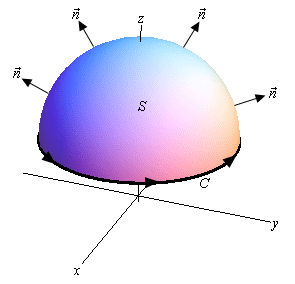
\includegraphics[width=50mm]{content/mvc/images/positive-oriented-boundary.png}
  \end{figure}
\end{definition}

\begin{namedtheorem}[Stoke's Theorem]
  Let $S$ be an oriented smooth surface, bounded by a curve $\partial S$, composed of finitely many simple closed smooth differentiable ($C^1$) curves with positive orientation. Let $\vec{F}$ be a differentiable ($C^1$) vector field whose domain includes $S$. Then
  \[
    \oint_{\partial S} \vec{F} \dotp d\vec{r} = \iint_S \del \crossp \vec{F} \dotp d\vec{S}
  \]

  In other words, the circulation of a vector field along a curve is the same as the sum of the curls within the surface bounded by the curve.
\end{namedtheorem}

\subsection{Gauss's Theorem}

\begin{namedtheorem}[Gauss's Theorem / Divergence theorem]
  Let $D$ be a solid region in $\Real^3$, bounded by a surface $\partial D$, composed of finitely many smooth closed surfaces with positive orientation. Let $\vec{F}$ be a differentiable ($C^1$) vector field whose domain includes $D$. Then
  \[
    \oiint_{\partial D} \vec{F} \dotp d\vec{S} = \iiint_D \del \dotp F dV
  \]

  In other words, the flux of a vector field through a closed surface is the same as the sum of the divergences of the vector field through the region bounded by the surface.

  This follows from that
  \begin{itemize}
    \item The ratio of flux to volume approaches the divergence as the volume becomes smaller.
    \item If the region is partitioned into smaller regions, the flux of the region is equal to the sum of the flux of the smaller regions (since the flux of the boundary of the two regions cancels out). 
  \end{itemize}
\end{namedtheorem}
